% Created 2024-07-12 Fri 16:28
% Intended LaTeX compiler: pdflatex
\documentclass{article}
\usepackage[utf8]{inputenc}
\usepackage[T1]{fontenc}
\usepackage{graphicx}
\usepackage{longtable}
\usepackage{wrapfig}
\usepackage{rotating}
\usepackage[normalem]{ulem}
\usepackage{amsmath}
\usepackage{amssymb}
\usepackage{capt-of}
\usepackage{hyperref}

\usepackage{fancyhdr}
\usepackage[top=25mm, left=25mm, right=25mm]{geometry}
\usepackage{longtable}
\fancyhead[R]{}
\setlength\headheight{43.0pt}
\author{Alexis Bautista}
\date{2024-07-23}
\title{Curso Esamblaje de Compuatodores}
\hypersetup{
 pdfauthor={Alexis Bautista},
 pdftitle={Curso Esamblaje de Compuatodores},
 pdfkeywords={},
 pdfsubject={},
 pdfcreator={Emacs 29.3 (Org mode 9.6.15)}, 
 pdflang={Español}}
\begin{document}

\maketitle
\fancyhead[C]{\includegraphics[scale=0.05]{./images/logoEPN.jpg}\\
ESCUELA POLITÉCNICA NACIONAL\\FACULTAD DE INGENIERÍA DE SISTEMAS\\
ARQUITECTURA DE COMPUTADORES}
\thispagestyle{fancy}

\section{Curso Completado:}
\label{sec:org50b67d3}

\begin{center}
\includegraphics[width=.9\linewidth]{./images/cursoCOmpletado.png}
\end{center}

\section{Módulo 1: Computadoras Personales}
\label{sec:org1fca212}

\begin{center}
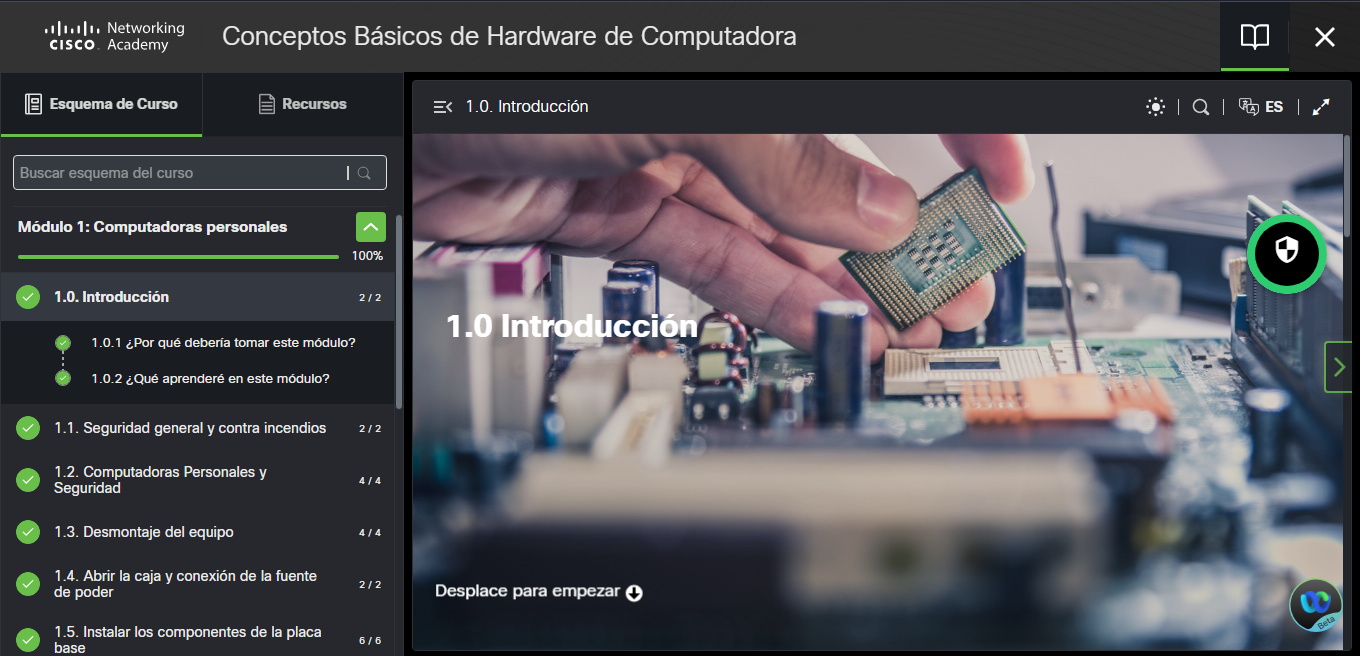
\includegraphics[width=.9\linewidth]{./images/modulo1.png}
\end{center}
\begin{center}
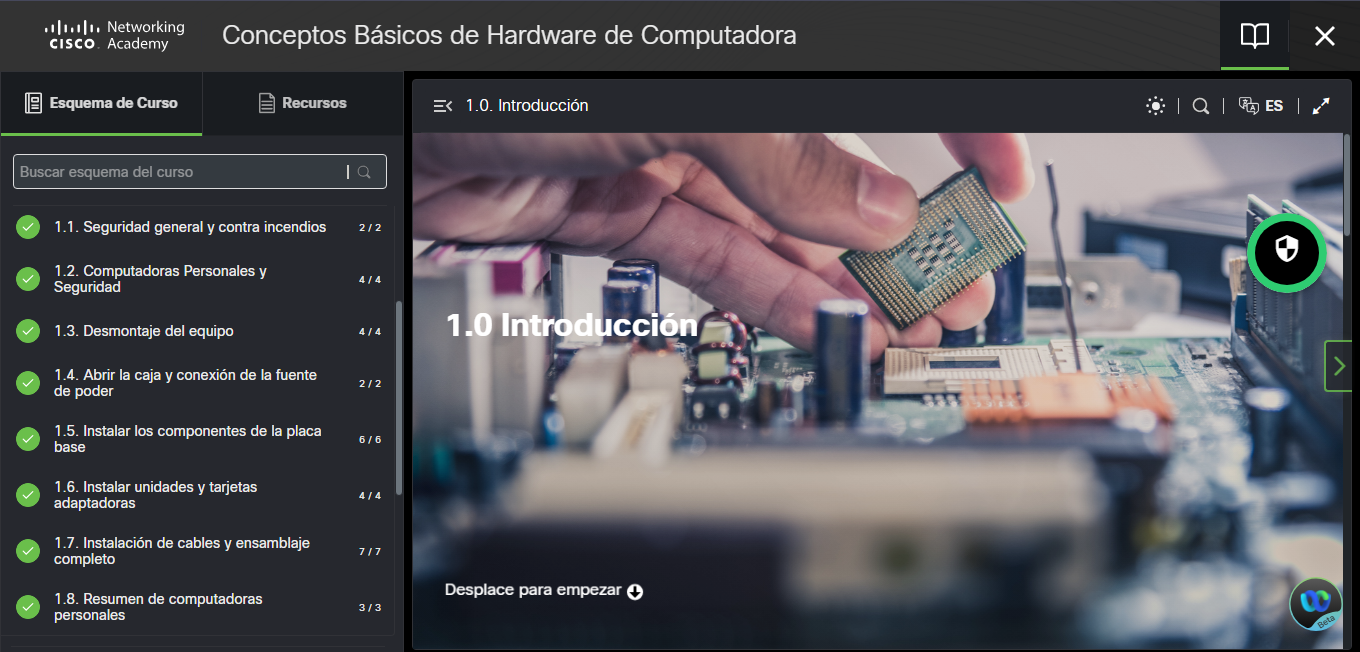
\includegraphics[width=.9\linewidth]{./images/modulo1_1.png}
\end{center}

\section{Módulo 2: Computadoras Portátiles}
\label{sec:org683a01b}

\begin{center}
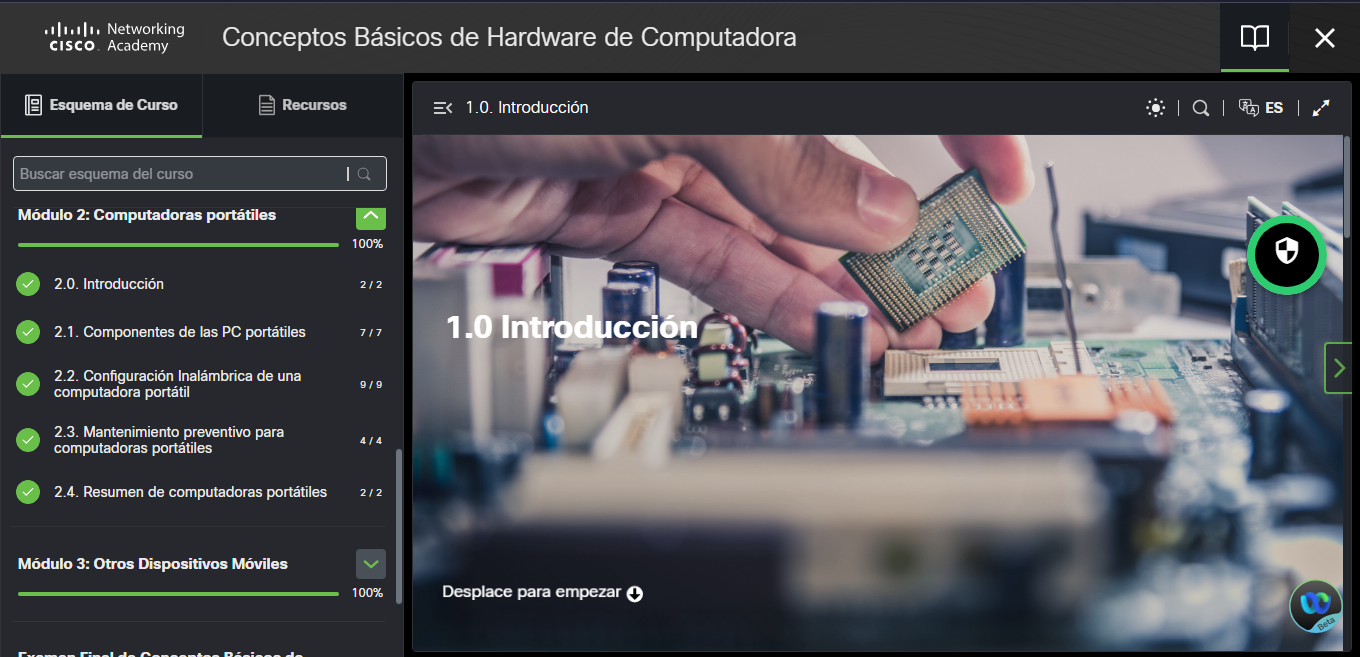
\includegraphics[width=.9\linewidth]{./images/modulo2.png}
\end{center}

\section{Módulo 3: Otros Dispositivos Moviles}
\label{sec:org04c6506}

\begin{center}
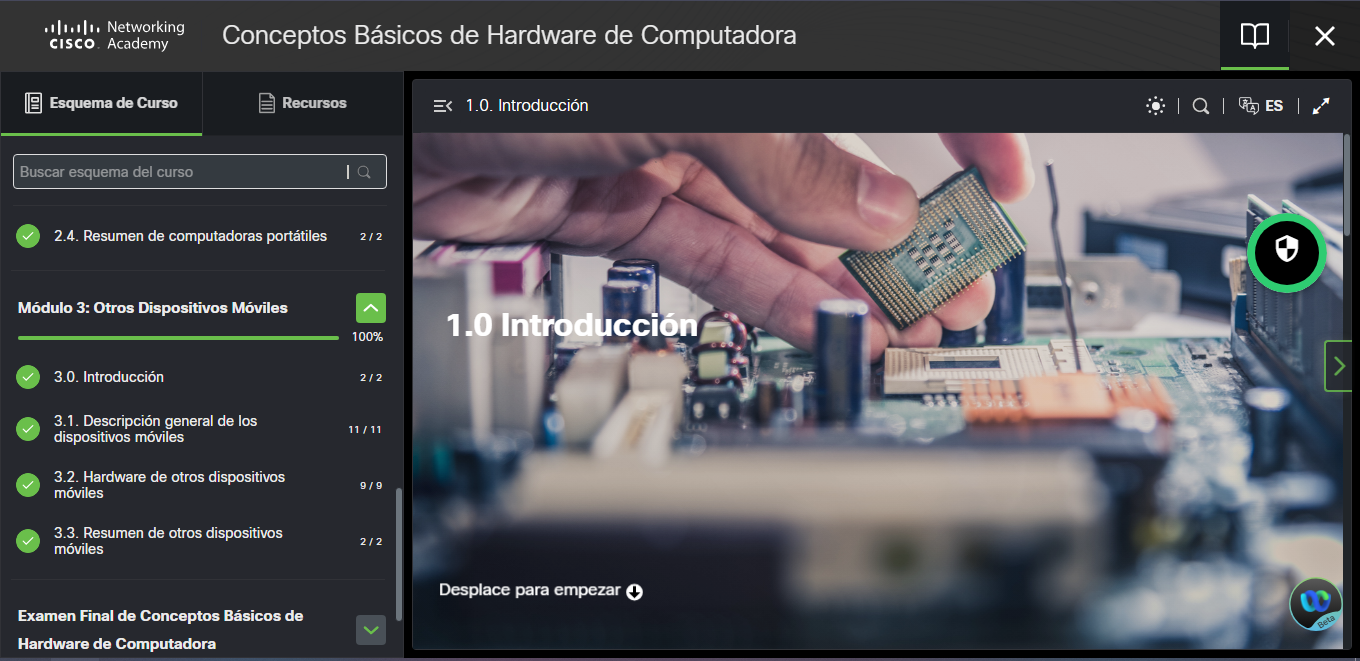
\includegraphics[width=.9\linewidth]{./images/modulo3.png}
\end{center}

\section{Examen Final}
\label{sec:org0686bb3}

\begin{center}
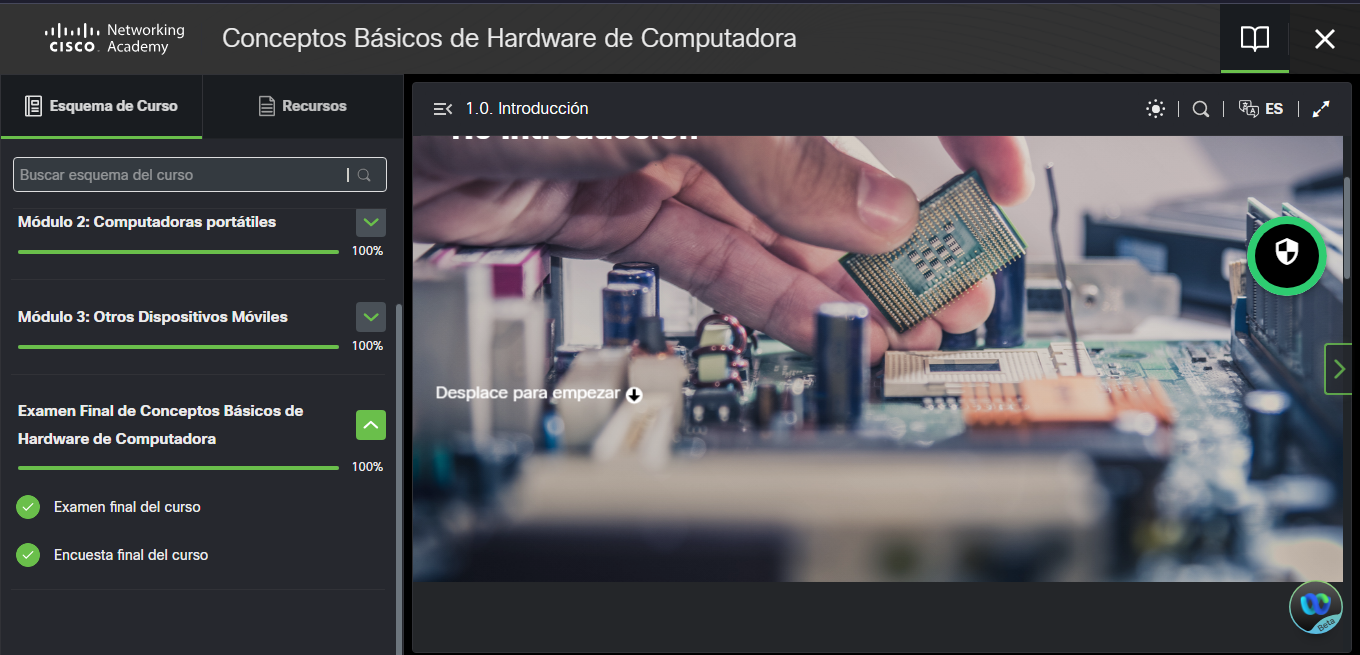
\includegraphics[width=.9\linewidth]{./images/examen.png}
\end{center}


\section{Comentarios:}
\label{sec:org538c6f4}

\begin{itemize}
\item Una de las cosas más importantes que me parecieron del curso son los
cuidados que debemos tener al manipular los componentes de un
computador u otro dispositivo electrónico. La electricidad estática,
por ejemplo, puede dañar los componentes, lo que puede resultar
costoso reponer.

Otra cosa importante es entender el funcionamiento de los
extintores, ya que este conocimiento puede ser útil incluso en otras
situaciones de emergencia.

\item También es esencial conocer todos los componentes de los
computadores y portátiles, así como su uso. Aunque los componentes
son similares para ambos, en los portátiles algunos varían, como las
memorias y CPUs, que son más pequeñas y consumen menos energía.

\item Cada día estamos más conectados y tenemos más dispositivos
interconectados, como relojes, tabletas, lectores electrónicos,
etc. Sin embargo, estos dispositivos no son fáciles de abrir para
limpiarlos internamente, pero podemos limpiarlos por fuera, teniendo
en cuenta no usar sustancias fuertes para las pantallas u otros
componentes. Además, es importante conocer el uso adecuado de estos
dispositivos.
\end{itemize}
\end{document}
